\documentclass[a4paper]{article}
\usepackage{exercise}
\usepackage{mathtools}

\usepackage{hyperref}

\title{\textbf{Robotics Summerschool Juli 2012} \\ Dag 3: Lopen met planning }
\author{Dutch Nao Team - \url{http://dutchnaoteam.nl}}
\date{}

\begin{document}
\maketitle

\section{Introductie}

Nu jullie A* planningsalgoritme af is zouden jullie de robot bij een willekeurige ingang kunnen zetten, en de robot intrueren om naar een willekeurige uitgang te lopen! Alleen weet de robot nog niet waar hij is in het doolhof. Jullie zouden net als bij dag 2 de kleurenmarkers kunnen gebruiken op de muur om zo te bepalen waar je bent.Zoals je misschien al hebt gemerkt zijn deze kleurenmarkers vrij instabiel. Vandaag gaan we met stabielere landmarks werken die in de robotica veel worden gebruikt. Dit zijn Augmented Reality (AR) codes. Op het middelpunt van elke vierkant in de grid leggen we zo een AR code neer. Zo kan de Nao altijd stabiel zien waar hij naartoe loopt.

\tableofcontents

\newpage

\section{AR codes}
AR codes zijn zwart-witte markers die een ID of `signature' in binaire code representeren. We hebben een lijstje met de AR codes die we gebruiken en hun ID bijgevoegd in dit document (scroll naar onder, 4 rijen). De AR codes zijn alleen zwart-wit zodat de overgangen tussen de lijnen makkelijk te herkennen zijn door een computer. Onze specifieke codes bestaan uit een 5x5 grid waarin elk vakje een binaire 1 of 0 aangeeft. Hieromheen zit een zwarte rand om de code makkelijk uit te kunnen lezen. Ze zijn vierkant met een vooraf gedefini\"eerde grootte zodat robots met wat goniometrie precies kunnen bepalen hoever ze van de AR code af staan. De draaiing van een camera ten opzichte van de code kan ook altijd uniek bepaald worden.

\begin{figure}[h]
\begin{center}$
\begin{array}{ccccc}
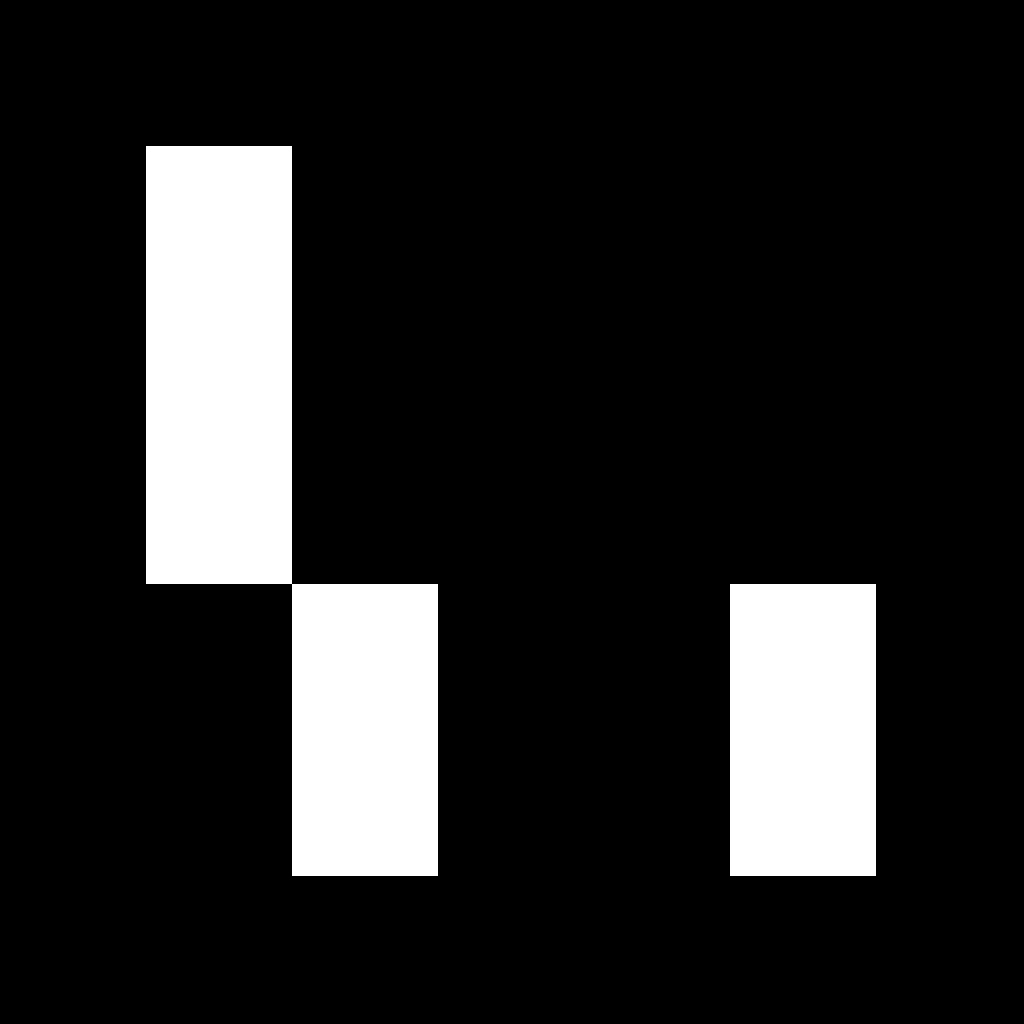
\includegraphics[width=0.8in]{10.jpg} &
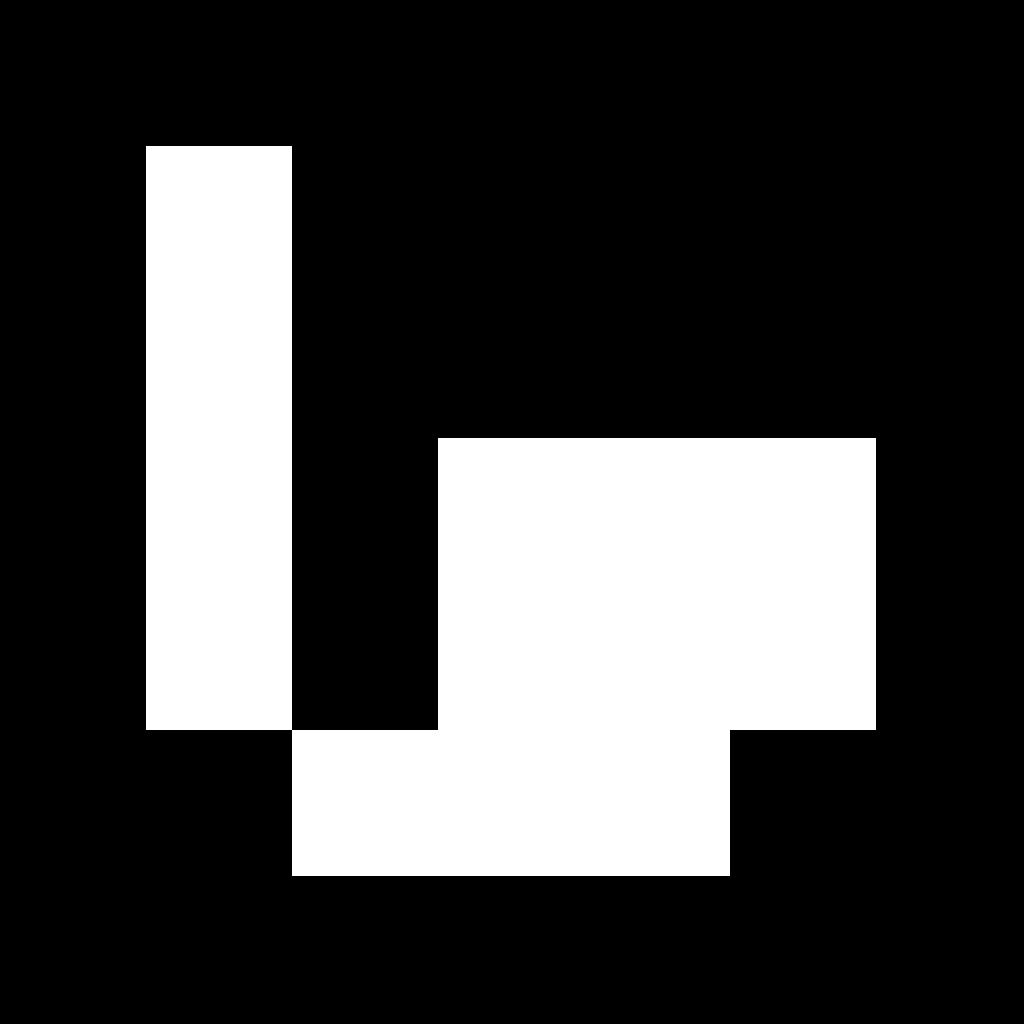
\includegraphics[width=0.8in]{23.jpg} &

\includegraphics[width=0.8in]{25.jpg} &
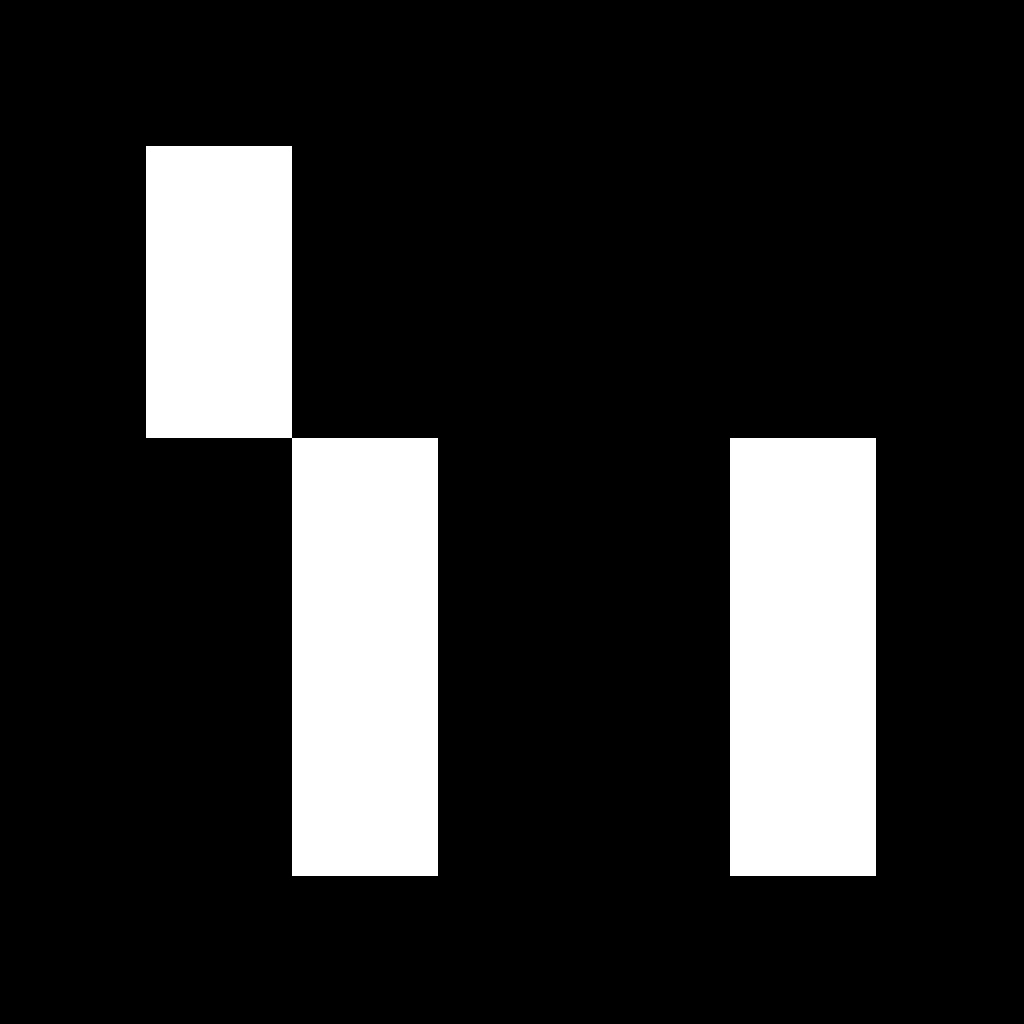
\includegraphics[width=0.8in]{42.jpg} &
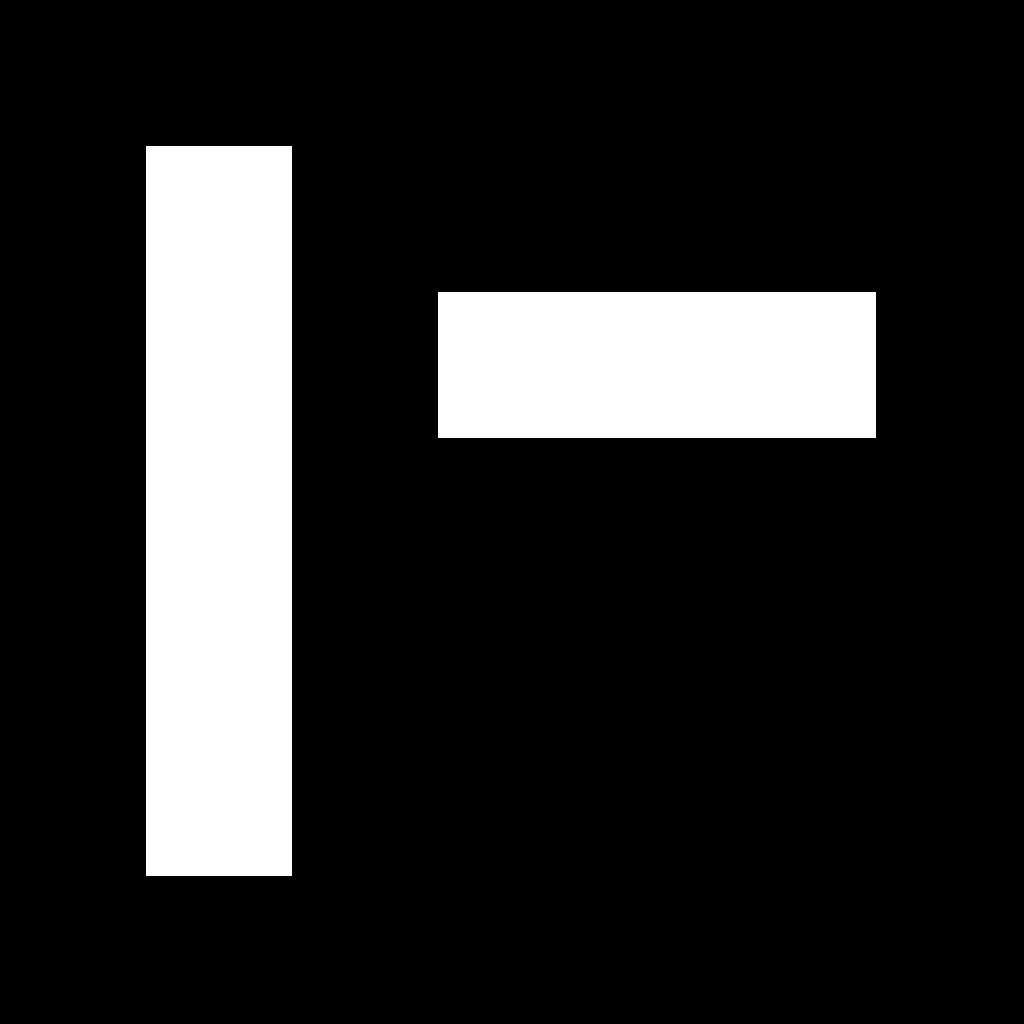
\includegraphics[width=0.8in]{64.jpg}
\end{array}$
\end{center}
\caption{AR codes (10, 23, 25, 42,64)}
\end{figure}

\begin{figure}[h]
\begin{center}$
\begin{array}{ccccc}

\includegraphics[width=0.8in]{69.jpg} &

\includegraphics[width=0.8in]{116.jpg} &

\includegraphics[width=0.8in]{123.jpg} &
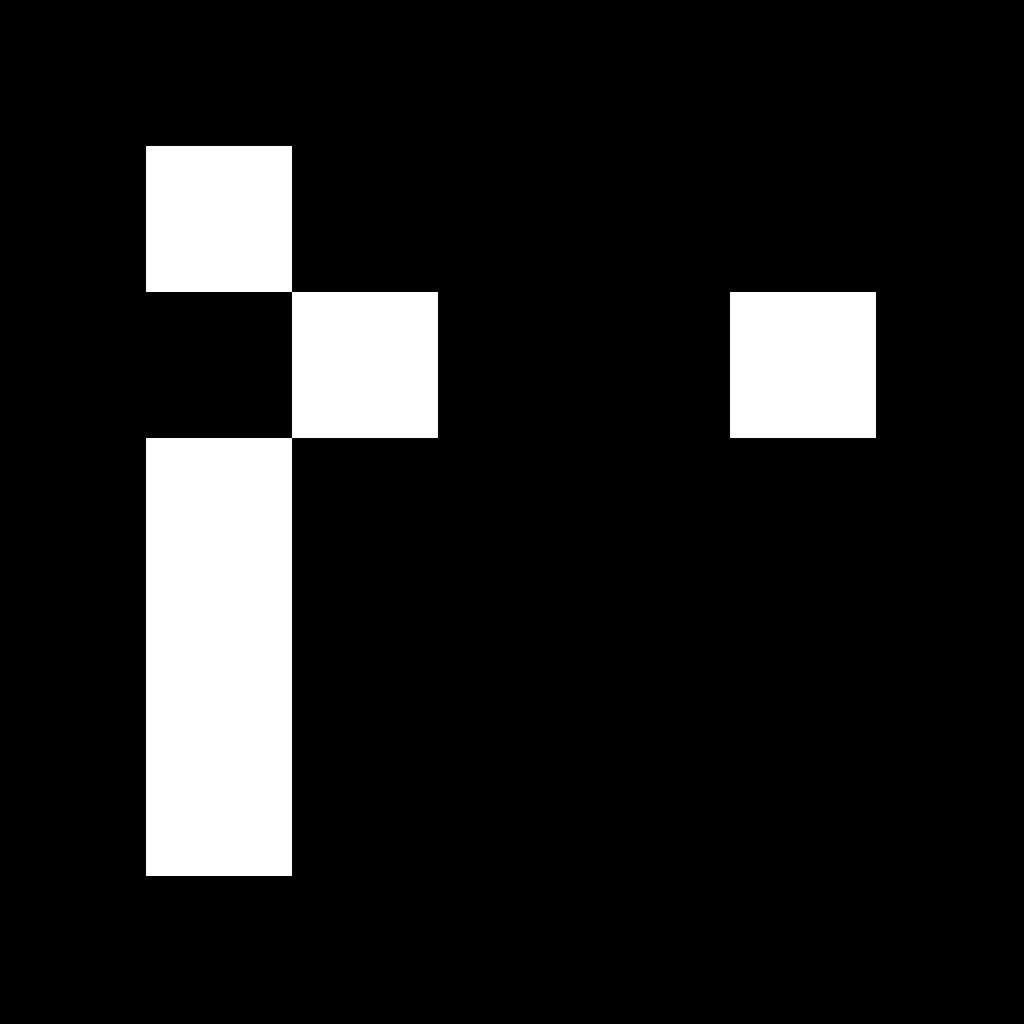
\includegraphics[width=0.8in]{128.jpg} &

\includegraphics[width=0.8in]{256.jpg}
\end{array}$
\end{center}
\caption{AR codes (69, 116, 123, 128, 256)}
\end{figure}

\begin{figure}[h]
\begin{center}$
\begin{array}{ccccc}

\includegraphics[width=0.8in]{444.jpg} &

\includegraphics[width=0.8in]{456.jpg} &

\includegraphics[width=0.8in]{501.jpg} &

\includegraphics[width=0.8in]{507.jpg} &
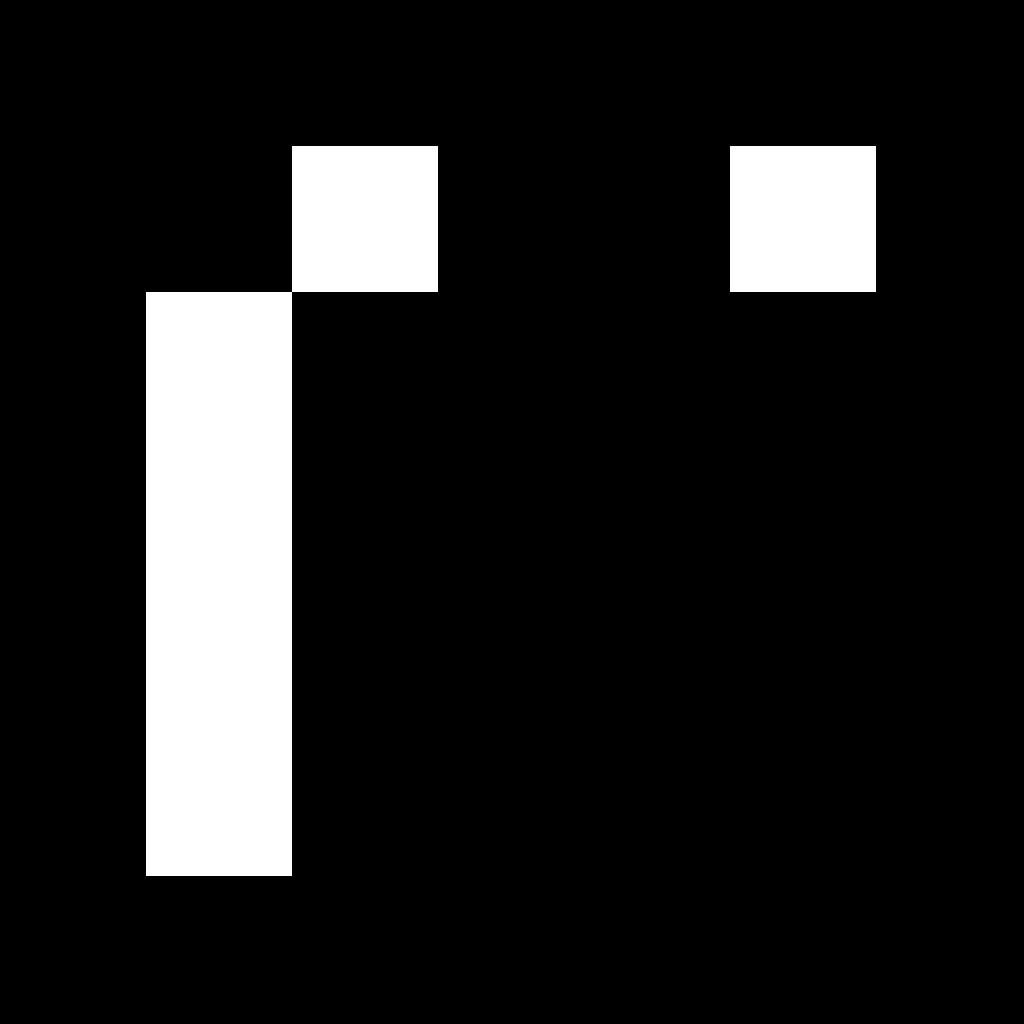
\includegraphics[width=0.8in]{512.jpg}
\end{array}$
\end{center}
\caption{AR codes (444, 456, 501, 507, 512)}
\end{figure}

\begin{figure}[h]
\begin{center}$
\begin{array}{ccccc}
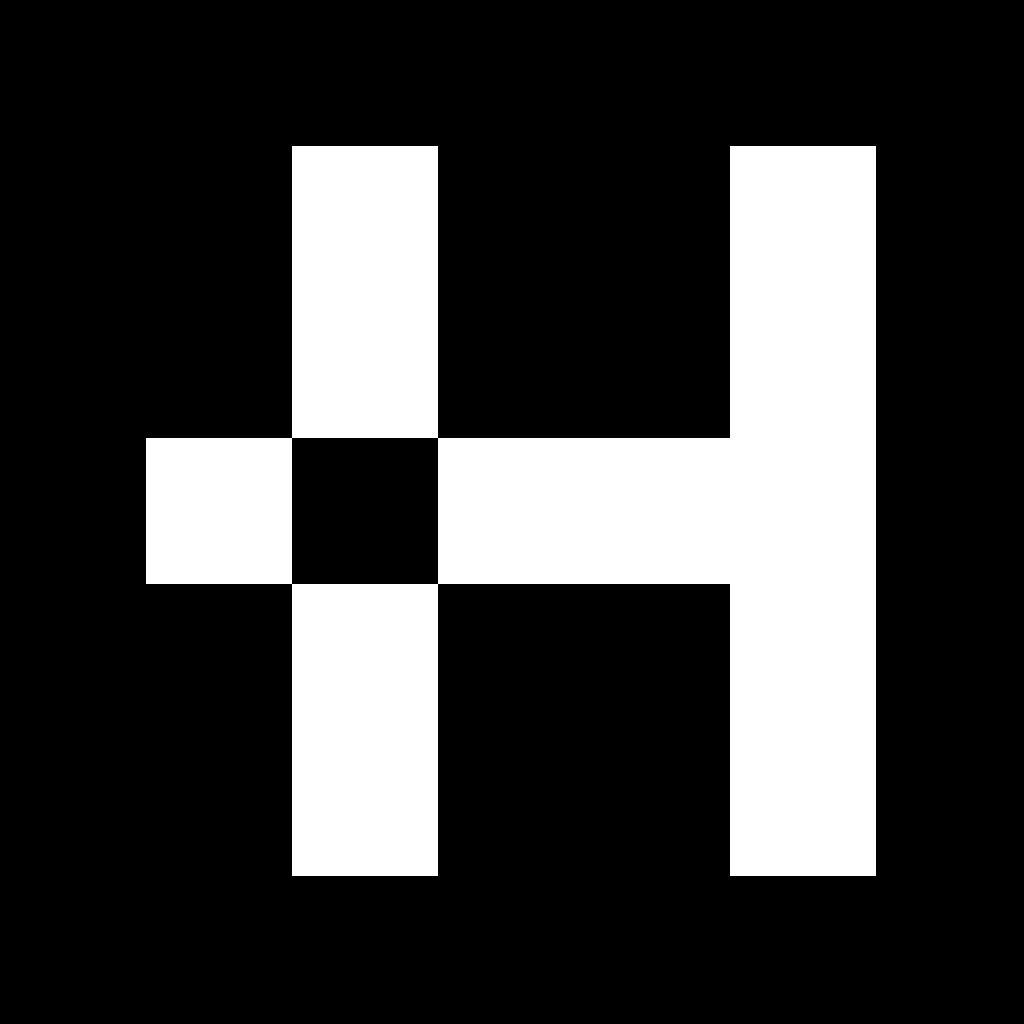
\includegraphics[width=0.8in]{666.jpg} &

\includegraphics[width=0.8in]{789.jpg} &

\includegraphics[width=0.8in]{890.jpg} &

\includegraphics[width=0.8in]{901.jpg} &

\includegraphics[width=0.8in]{999.jpg}
\end{array}$
\end{center}
\caption{AR codes (666, 789, 890, 901,999)}
\end{figure}

\section{AR code code}
Net zoals de OpenCV code die jullie hebben gebruikt is de code om AR codes te herkennen geschreven in C$ \stackrel{}{++}$. Dit hebben we gedaan omdat Python doorgaans niet snel genoeg is voor computer vision. Als je het leuk vind om te weten wat hier allemaal bij komt kijken, vraag dit dan gerust aan Tijmen (die jongen met de oranje haren).

\begin{Exercise}
Download de ARCodeTest zip van onze server, en pak deze uit. Kijk in de map die je hebt uitgepakt.
\end{Exercise}
\vspace{10 mm}
De specifieke rekencore van de AR code detectie zit in de dynamic link library file aruco124.dll. Hiervoor hebben we een python interface geschreven die zich bevind in \_ARimport.pyd en ARimport.py. De code in ARimport.py is zeker weten niet bedoeld om te lezen. Wat wel bedoeld is om te lezen is de ARtest.py file. Hier staat eigenlijk alles in wat je nodig hebt om AR markers te kunnen herkennen

\begin{Exercise}
 Draai de ARtest.py file en kijk naar de output. Wat is er gebeurd tussen de twee plaatjes? Heeft hij de marker goed herkend?
\end{Exercise}
\vspace{10 mm}

Schrik niet dat er een regeltje output in je python scherm komt, deze kan je gewoon negeren. Dit komt door het omzetten van de C$\stackrel{}{++}$ naar Python code. 
We gaan de code nu een stap voor stap ontleden. Als eerste moeten de modules cv en cv2 geinclude worden (d\'e standaard voor computer vision AI software). Daarnaast gaan we numpy nodig hebben, dit is een python library die ervoor zorgt dat numerieke code met matrices erg snel uitgevoerd kan worden. Ook moeten we natuurlijk een AR code detectie class importen. Dit gebeurd in de eerste 4 regels van ARtest.py. Wat er op de andere regels gebeurd staat hier en in de code uitgelegd.
\begin{itemize}
\item \emph{ARcode = ar.ARimport()} maken we een nieuw ARcode object aan. Tegelijk initialiseert deze regel ook dit object met al zijn nodige waardes.
\item \emph{image = cv.LoadImage("test.png",cv.CV\_LOAD\_IMAGE\_COLOR)} Laad het opencv testplaatje als kleurenplaatje
\item \emph{im\_array = np.asarray( image[:,:] ) } Om het plaatje naar de C$\stackrel{}{++}$ te kunnen sturen moeten we er een numpy array van maken.
\item{ARcode.setOutputFileName("output.png") / ARcode.setShowOutput(True)} Met deze regels zetten we de output van de library aan. Deze kan je in je uiteindelijke implementatie gewoon uit laten.
\item{returnint = ARcode.findMarkers(im\_array)} Als je deze functie aanroept gaat ARcode de markers berekenen, deze worden lokaal opgeslagen in de ARcode class. Hij returned een integer die aangeeft hoeveel markers er zijn gevonden.
\item{output = ARcode.getFoundMarker(0)} Deze functie geeft de informatie van de gevonden marker. Het getal dat je meegeeft is het nummer van de marker waar je de informatie van opvraagd. Dit getal mag niet groter zijn dan `returnint' dan crasht de applicatie gegarandeerd. met output.ID, output.x en output.y kan je de ID van de gevonden marker en de x en y positie in het gegeven plaatje van het midden van de marker vinden.
\end{itemize}

\begin{Exercise}
Maak zelf wat plaatjes met 1 of meer AR codes erin en test hoe robuust de AR codes gevonden kunnen worden, hoeveel maakt het uit als je ze bekijkt onder verschillende hoeken? Hoe maak je het opvragen van de gevonden AR codes veilig (dat hij niet crasht?). 
\end{Exercise}
\vspace{10 mm}

\section{Omgaan met de markers}

Nu kan je makkelijk AR markers vinden in plaatjes, dit maakt de computer vision op de Nao een stuk makkelijker! Het enige wat je nu nog nodig hebt is een vertaalstap van de x,y waardes in het plaatje naar de x,y waardes in de echte wereld.. Dit is natuurlijk nodig om de Nao naar de marker toe te laten lopen. Hiervoor hebben we de functie tools.calcPosition(x\_in\_image,y\_in\_image) in de tools module. Dit is een slimme functie die met behulp van de hoogte informatie van de nao, en de informatie dat de AR code op de grond ligt (!) berekent wat de echte x,y afstand is met als input de x en y waardes uit het plaatje. De functie neemt ook de draaiïng van het hoofd van de Nao mee, dus als de Nao zijn hoofd draait naar een marker dan is de output (x,y) nog steeds precies wat de Nao hoort te lopen om op de marker te komen (jammer genoeg loopt hij nog steeds niet zo heel accuraat).

\begin{Exercise}
\begin{itemize}
\item Schrijf nu een functie in een nieuwe dag 3 module waar je een plaatje van de Nao aan mee kan geven, en een lijst met informatie over alle markers teruggeeft. (bijvoorbeeld [(x\_1,y\_1,ID\_1), (x\_1,y\_1,ID\_1)]).
\item Schrijf een functie die het hoofd van de Nao laat draaien naar een marker (input (x\_1,y\_1,ID\_1))
\item Schrijf een functie die een Nao op een marker af laat lopen.
\item Voeg alle ID markers op nummer toe aan de representatie van het doolhof. Of controleer of we dit al gedaan hebben
\item Test of al deze functies goed werken!
\end{itemize}
\end{Exercise}
\vspace{10 mm}



\section{Volledige autonome navigatie}

Je hebt nu alle tools om de Nao geheel zelfstandig door het doolhof te laten lopen! Met A* kan de Nao een pad plannen, en met de AR markers weet de Nao waar hij is en kan je hem eenvoudig laten lopen. Het enige dat de Nao nodig heeft is zijn beginpositie en de gewenste eindpositie.

\begin{Exercise}
\begin{itemize}
\item Schrijf nu een main waarbij je zelf een beginpunt en eindpunt op kan geven, de Nao uit zichzelf het pad berekend vanuit het begin naar het einde, en deze dan ook loopt met behulp van de AR markers. Je mag zelf verzinnen hoe je dit slim kan doen. (Als je rotatie/translatie informatie van de AR-markers wil hebben hiervoor moet je dit aan Tijmen vragen).
\item Probeer je functie uit met verschillende begin- en eindpunten, vertel ons of je het werkend hebt gekregen, dat is namelijk echt een geweldige prestatie!
\item Als je nog tijd over heben we een final challenge. De nao word hierbij op een random punt in het doolhof gezet en hij moet zelf bepalen waar hij is, en hoe hij van dat punt naar de opgegeven uitgang moet lopen. Denk er goed over na hoe de Nao kan bepalen waar hij is, en hoe hij gedraaid staat. Wat doe je als de Nao helemaal geen marker ziet?
\end{itemize}
\end{Exercise}
\vspace{10 mm}

\end{document}